\chapter[Sprint II]{Study and Implementation of Sprint II: Authentication \& Landing Page}

\section{Introduction}
Sprint II focuses on developing the authentication system and landing page using NextAuth.js and Prisma ORM. This sprint establishes essential user management capabilities and creates an intuitive entry point for the application, building upon the foundation from previous iterations.

\section{Sprint Planning}

\subsection{Objectives}
\begin{itemize}
    \item Implement secure OAuth authentication (Google, GitHub)
    \item Develop cross-device session management
    \item Create responsive landing page
    \item Establish database schema with Prisma ORM
    \item Ensure seamless sign-in/sign-out functionality
\end{itemize}
\subsection{Backlog Items}

The MoSCoW prioritization method categorizes requirements into four levels: \textbf{Must have} (critical features essential for project success), \textbf{Should have} (important features that add significant value but aren't critical), \textbf{Could have} (nice-to-have features that can be included if time and resources allow), and \textbf{Won't have} (features explicitly excluded from current scope).

This method helps teams focus on delivering the most valuable features first while maintaining clear expectations about what will and won't be included in each release.

\begin{table}[H]
\centering
\caption{Sprint II Backlog}
\begin{tabular}{|p{1cm}|p{7cm}|p{2cm}|p{2cm}|}
\hline
\textbf{ID} & \textbf{User Story} & \textbf{Priority} \\
\hline
1 & As a user, I want to sign in with Google account & M\\
\hline
2 & As a user, I want to sign in with GitHub account & M\\
\hline
3 & As a user, I want to stay authenticated across devices & M\\
\hline
4 & As a user, I want to sign out from my account & S\\
\hline
5 & As a visitor, I want to explore the landing page & M\\
\hline
\end{tabular}
\end{table}
\section{System Analysis}

\subsection{Use Case Overview}
\begin{figure}[H]
    \centering
    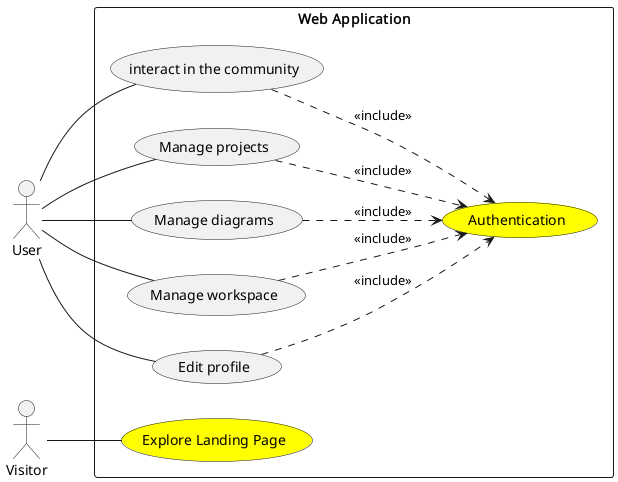
\includegraphics[width=0.8\textwidth]{conception/SprintII/use_case_diagrams/use_case_diagram_of_SprintII.png}
    \caption{Sprint II Use Case Diagram}
    \label{fig:usecase_sprint2}
\end{figure}
\newpage
\subsection{Authentication Use Cases}
\begin{figure}[H]
    \centering
    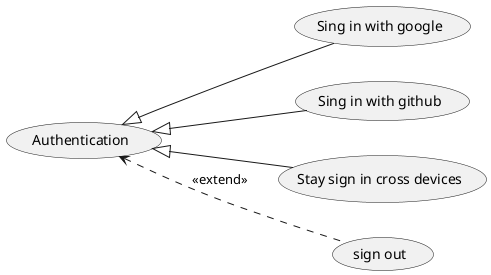
\includegraphics[width=0.8\textwidth]{conception/SprintII/use_case_diagrams/refined_use_case_feature_auth.png}
    \caption{Refined Authentication Use Case}
    \label{fig:refined_auth_usecase}
\end{figure}

\subsubsection{Core Authentication Scenarios}

\textbf{OAuth Sign-In Process:}
\begin{enumerate}
    \item User clicks OAuth provider button (Google/GitHub)
    \item System redirects to provider's authorization page
    \item User authorizes application access
    \item Provider returns authorization code
    \item System validates and creates user session
    \item User is redirected to dashboard
\end{enumerate}

\textbf{Cross-Device Authentication:}
Session persistence is maintained through secure tokens allowing users to access the application across multiple devices without re-authentication, with automatic session validation and expiration handling.

\textbf{Secure Sign-Out:}
Session termination involves token invalidation, cookie clearing, and secure redirection to the landing page.

\section{System Design}

\subsection{Authentication Flow}
\begin{figure}[H]
    \centering
    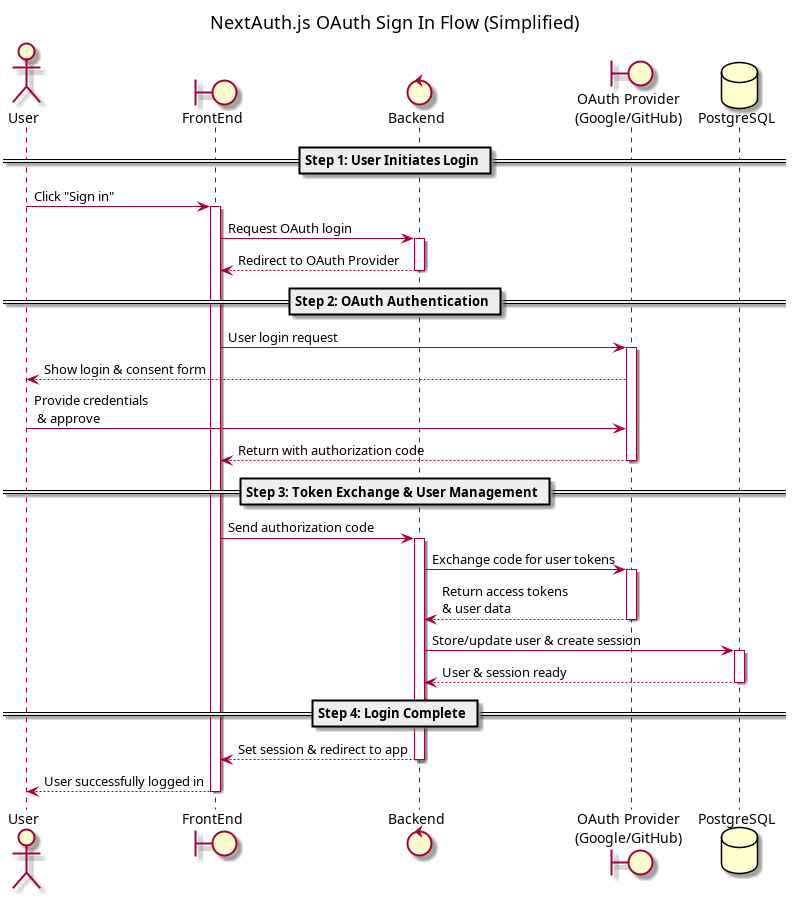
\includegraphics[width=0.8\textwidth]{conception/SprintII/sequence_diagrams/sequence_authentication_1_1_AuthenticateUsingGoogleAccount.png}
    \caption{OAuth Authentication Sequence}
    \label{fig:seq_google_auth}
\end{figure}


\section{Implementation Results}

\subsection{Landing Page}
\begin{figure}[H]
    \centering
    \includegraphics[width=1.0\textwidth]{screenshots/landing.png}
    \caption{Responsive Landing Page}
    \label{fig:landing_page}
\end{figure}

Modern design featuring clear value proposition, feature highlights, and prominent call-to-action elements optimized for user engagement and conversion.

\subsection{Authentication Interface}
\begin{figure}[H]
    \centering
    \includegraphics[width=0.8\textwidth]{screenshots/signin.png}
    \caption{OAuth Sign-In Interface}
    \label{fig:signin_page}
\end{figure}

Clean, user-friendly authentication interface supporting multiple OAuth providers with consistent branding and accessibility standards.

\section{Sprint Retrospective}

\textbf{Achievements:}
\begin{itemize}
    \item Successful OAuth integration with Google and GitHub
    \item Robust cross-device session management
    \item Responsive landing page with high conversion potential
    \item Secure authentication flow with proper error handling
\end{itemize}

\textbf{Challenges Resolved:}
\begin{itemize}
    \item OAuth configuration complexities across environments
    \item Session persistence optimization
    \item Cross-browser compatibility testing
\end{itemize}

\section{Conclusion}

Sprint II successfully established the authentication infrastructure and user entry point. The implementation of NextAuth.js with OAuth providers and Prisma database management provides a secure, scalable foundation for user management. The responsive landing page effectively communicates value while guiding user engagement. These achievements create a solid foundation for subsequent development phases, with robust security and optimal user experience.